\documentclass[./memory.tex]{subfiles}

\begin{document}
\chapter{Results}
In final chapter, the focus is on presenting the final results achieved in the
project. A set of images is provided to give an overview of the final outcomes,
showcasing both the desktop and mobile designs of the application.
\begin{figure}[H]
	\centering
	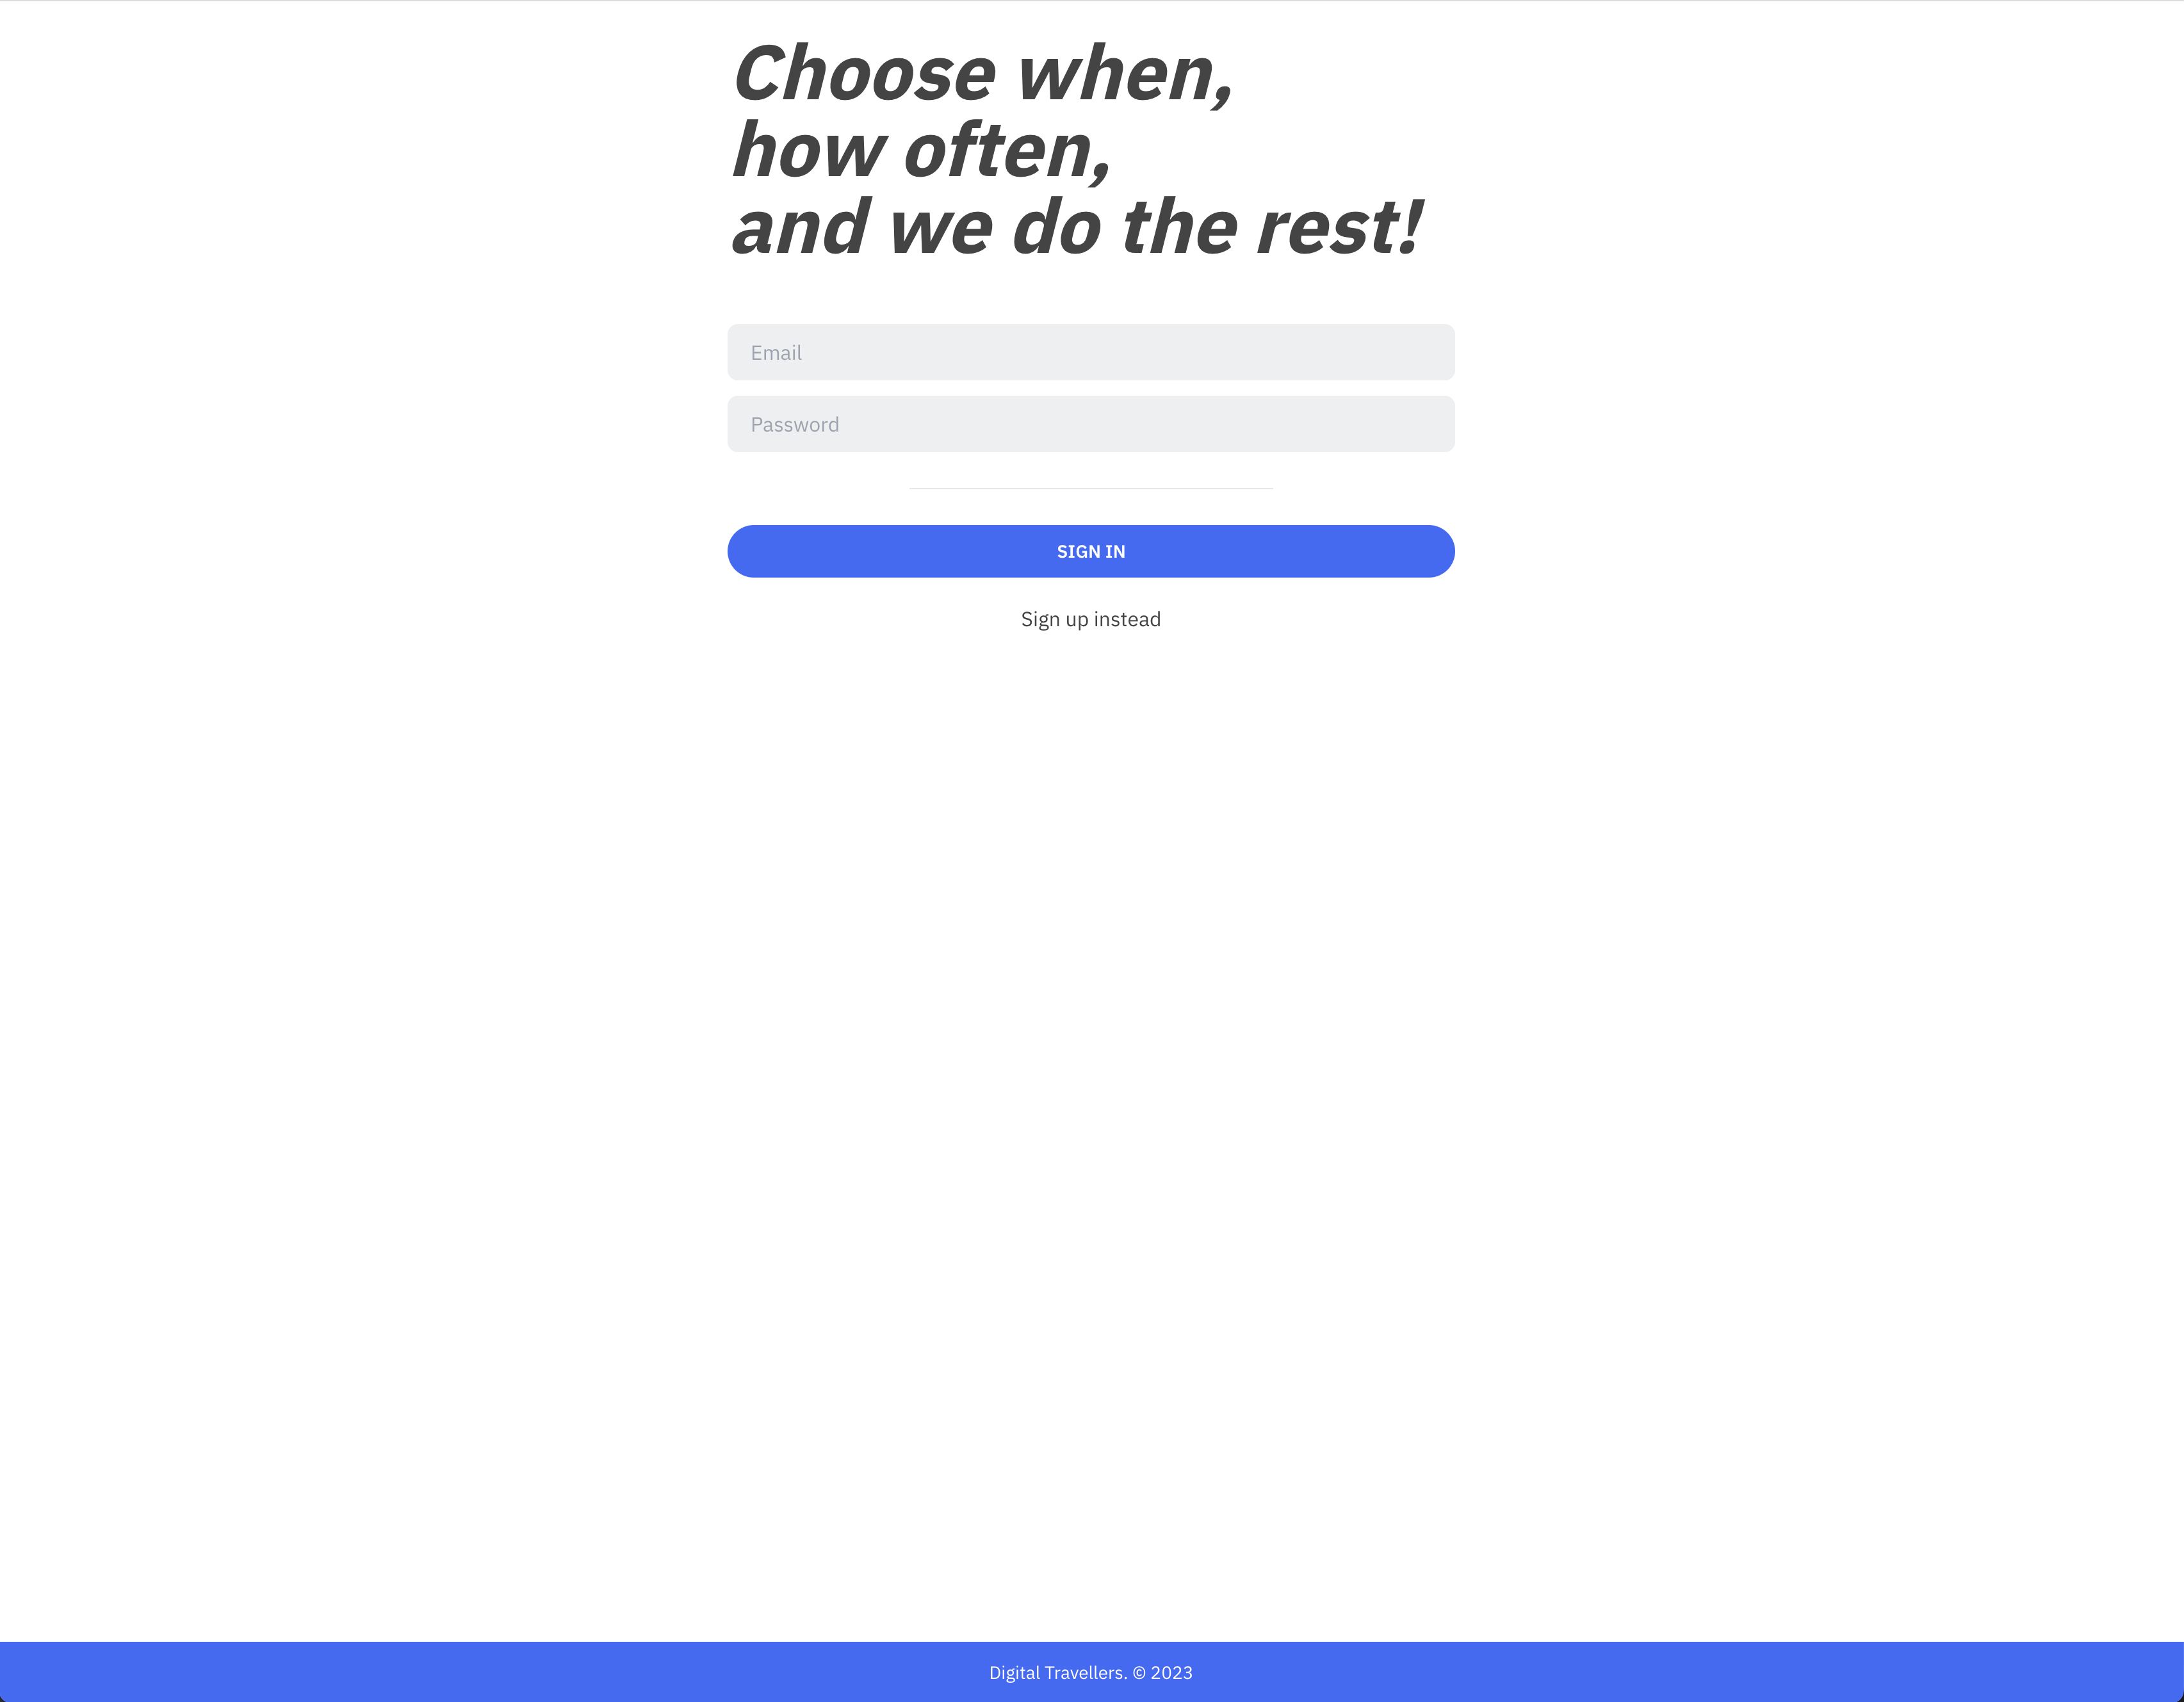
\includegraphics[width=\textwidth]{./assets/results/desktop-sign-in.png}
	\caption{Final result of the sign-in page for desktop devices}
\end{figure}
\begin{figure}[H]
	\centering
	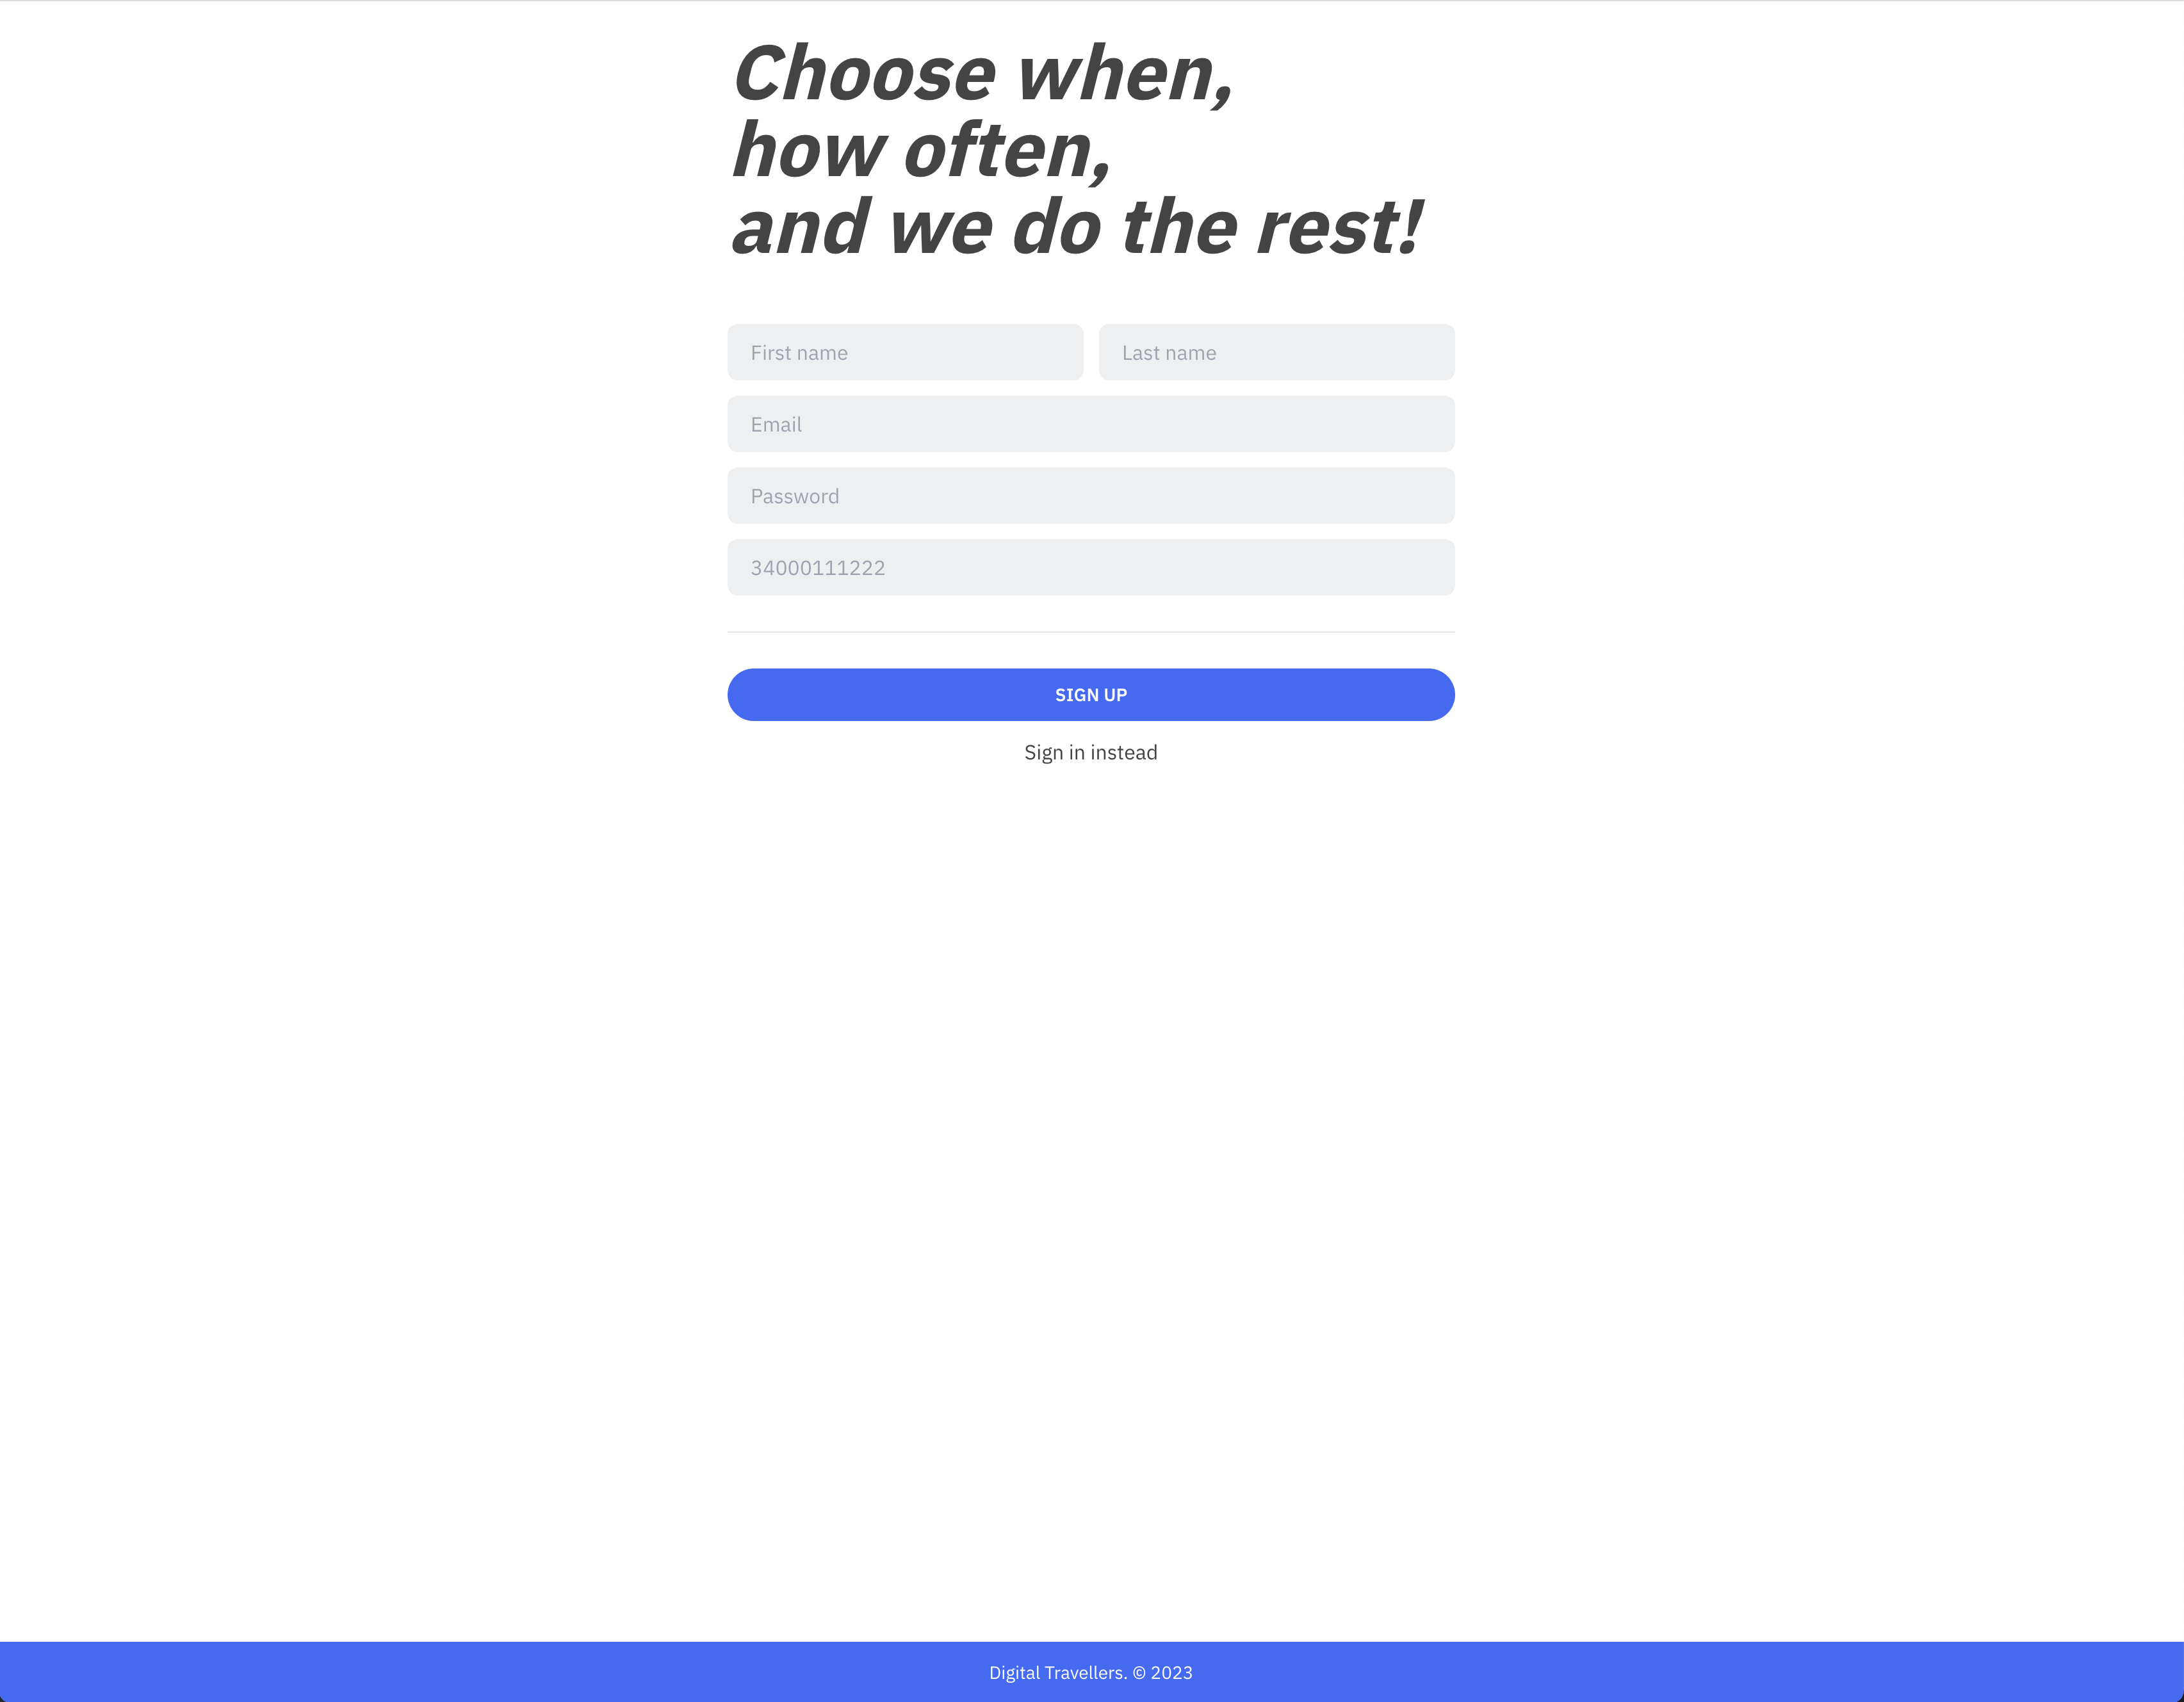
\includegraphics[width=\textwidth]{./assets/results/desktop-sign-up.png}
	\caption{Final result of the sign-up page for desktop devices}
\end{figure}
\begin{figure}[H]
	\centering
	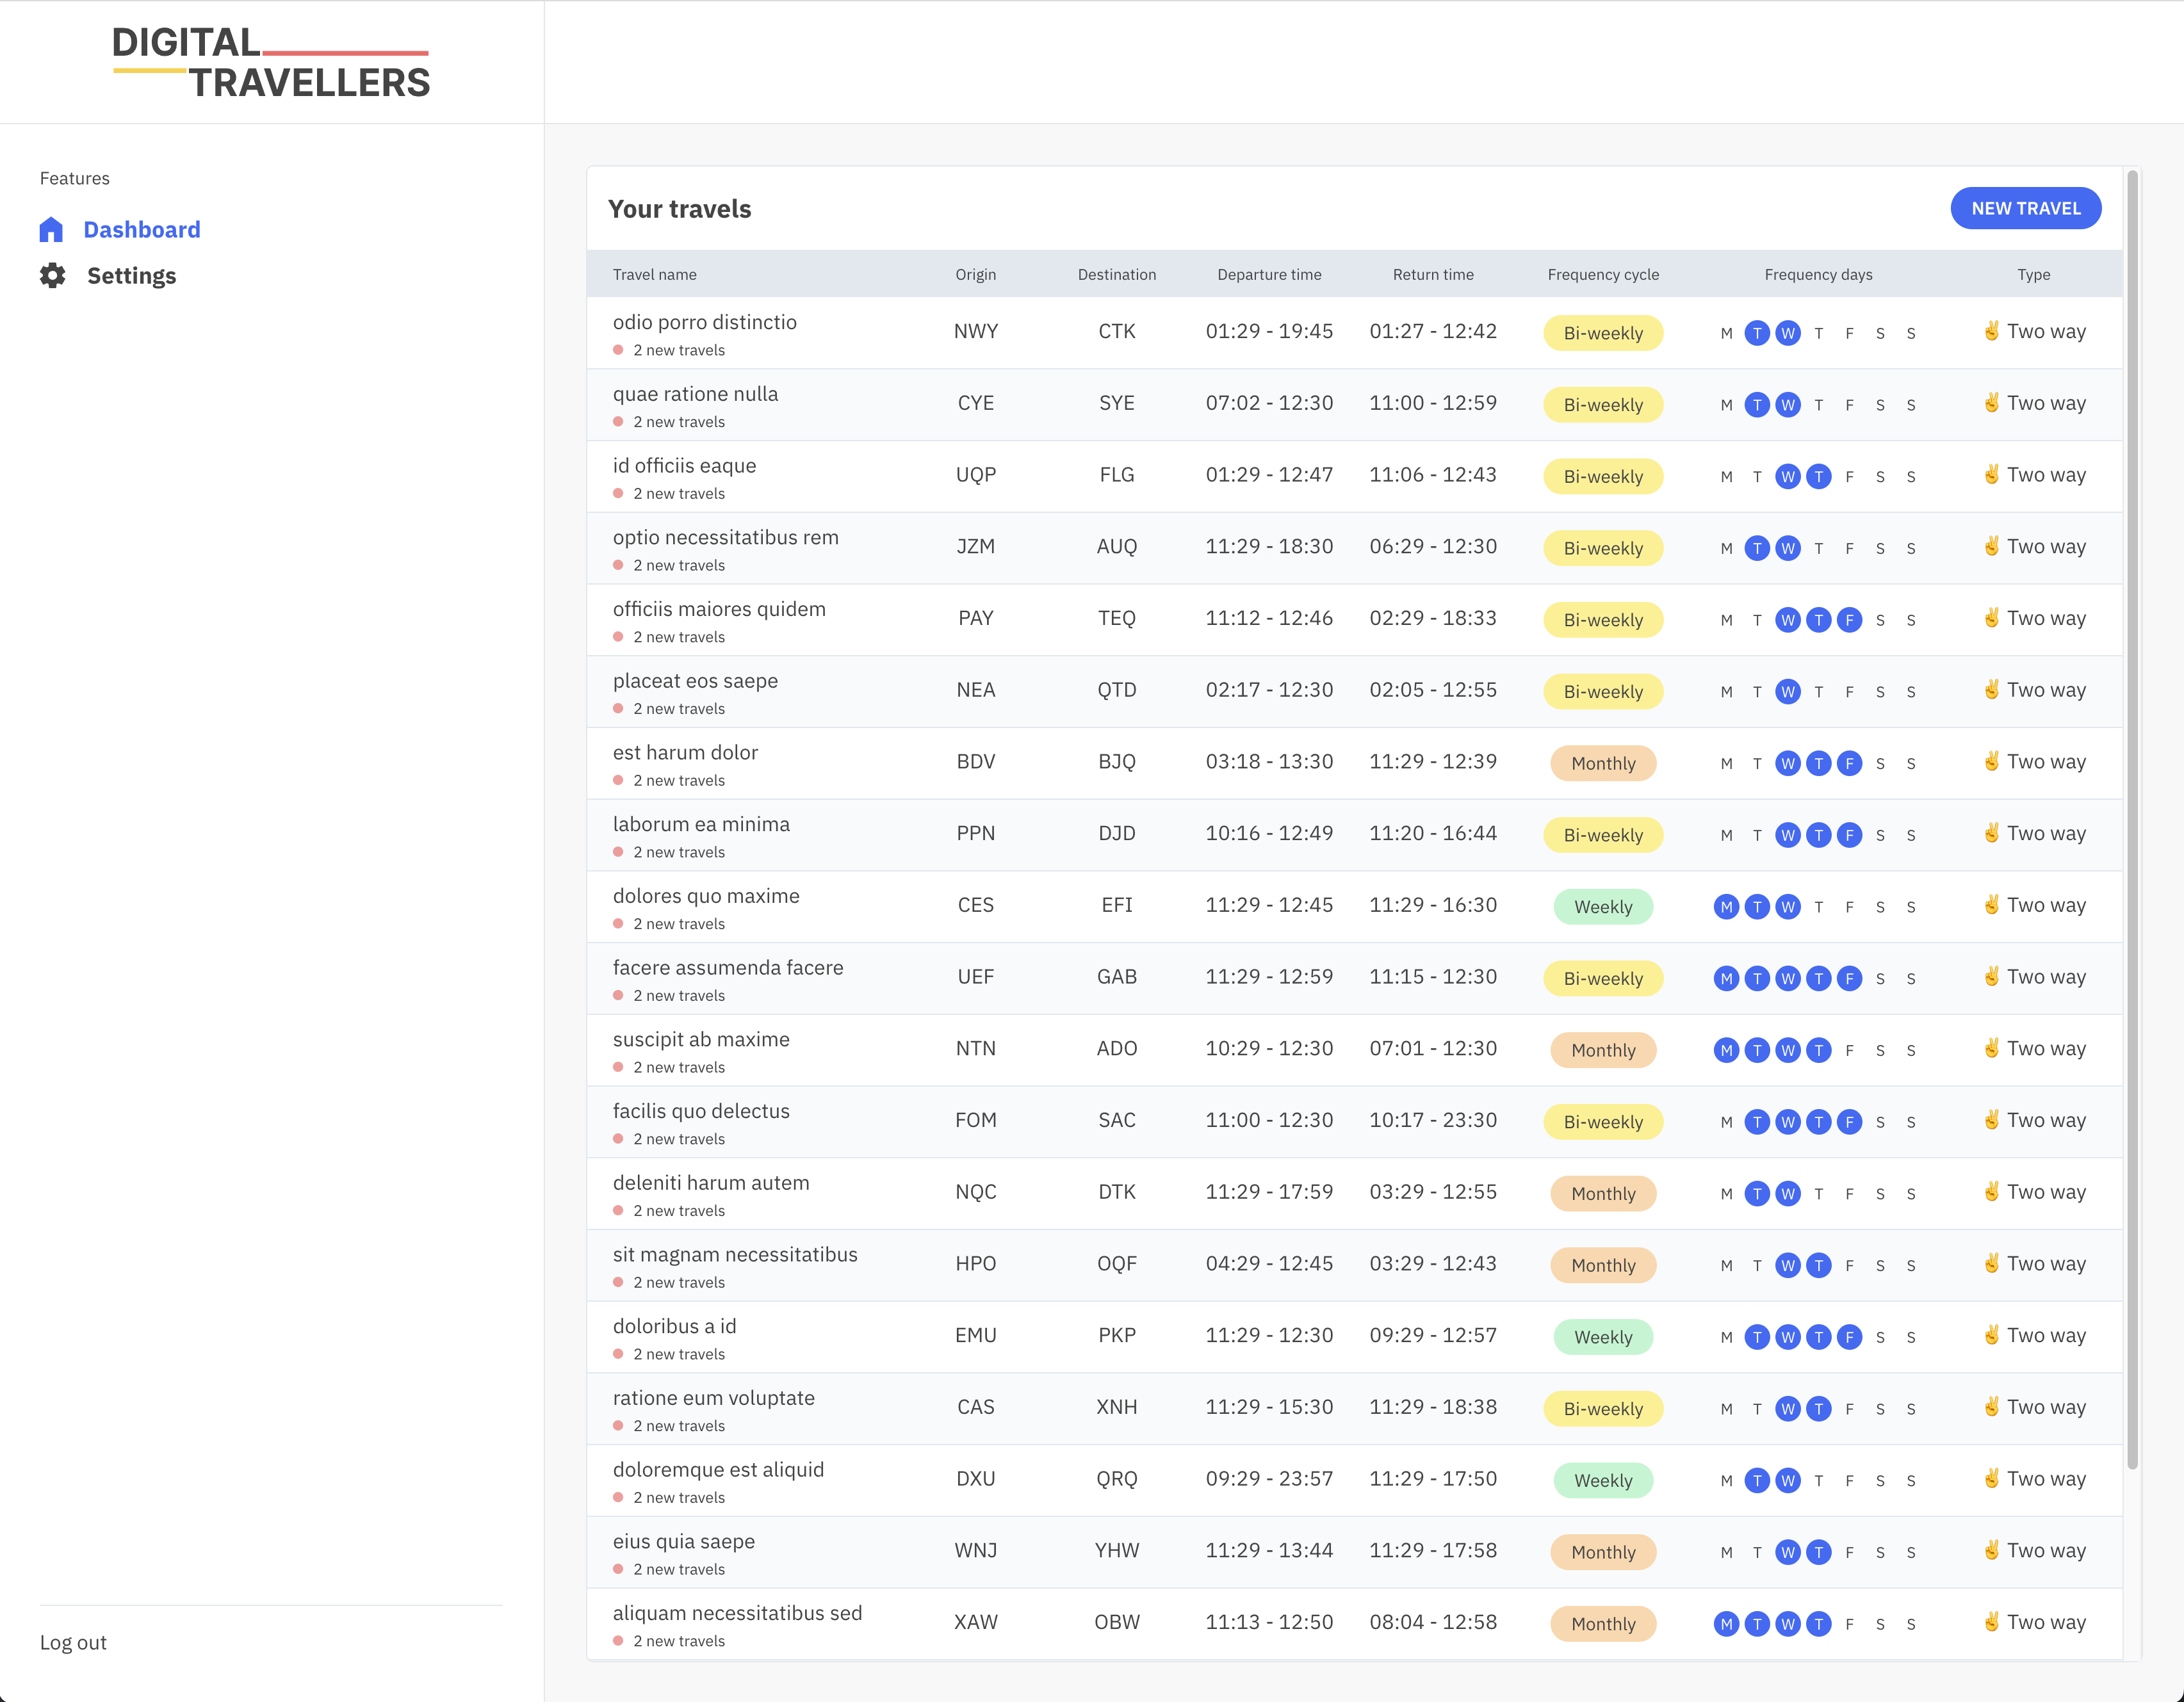
\includegraphics[width=\textwidth]{./assets/results/desktop-dashboard.png}
	\caption{Final result of the dashboard page for desktop devices}
\end{figure}
\begin{figure}[H]
	\centering
	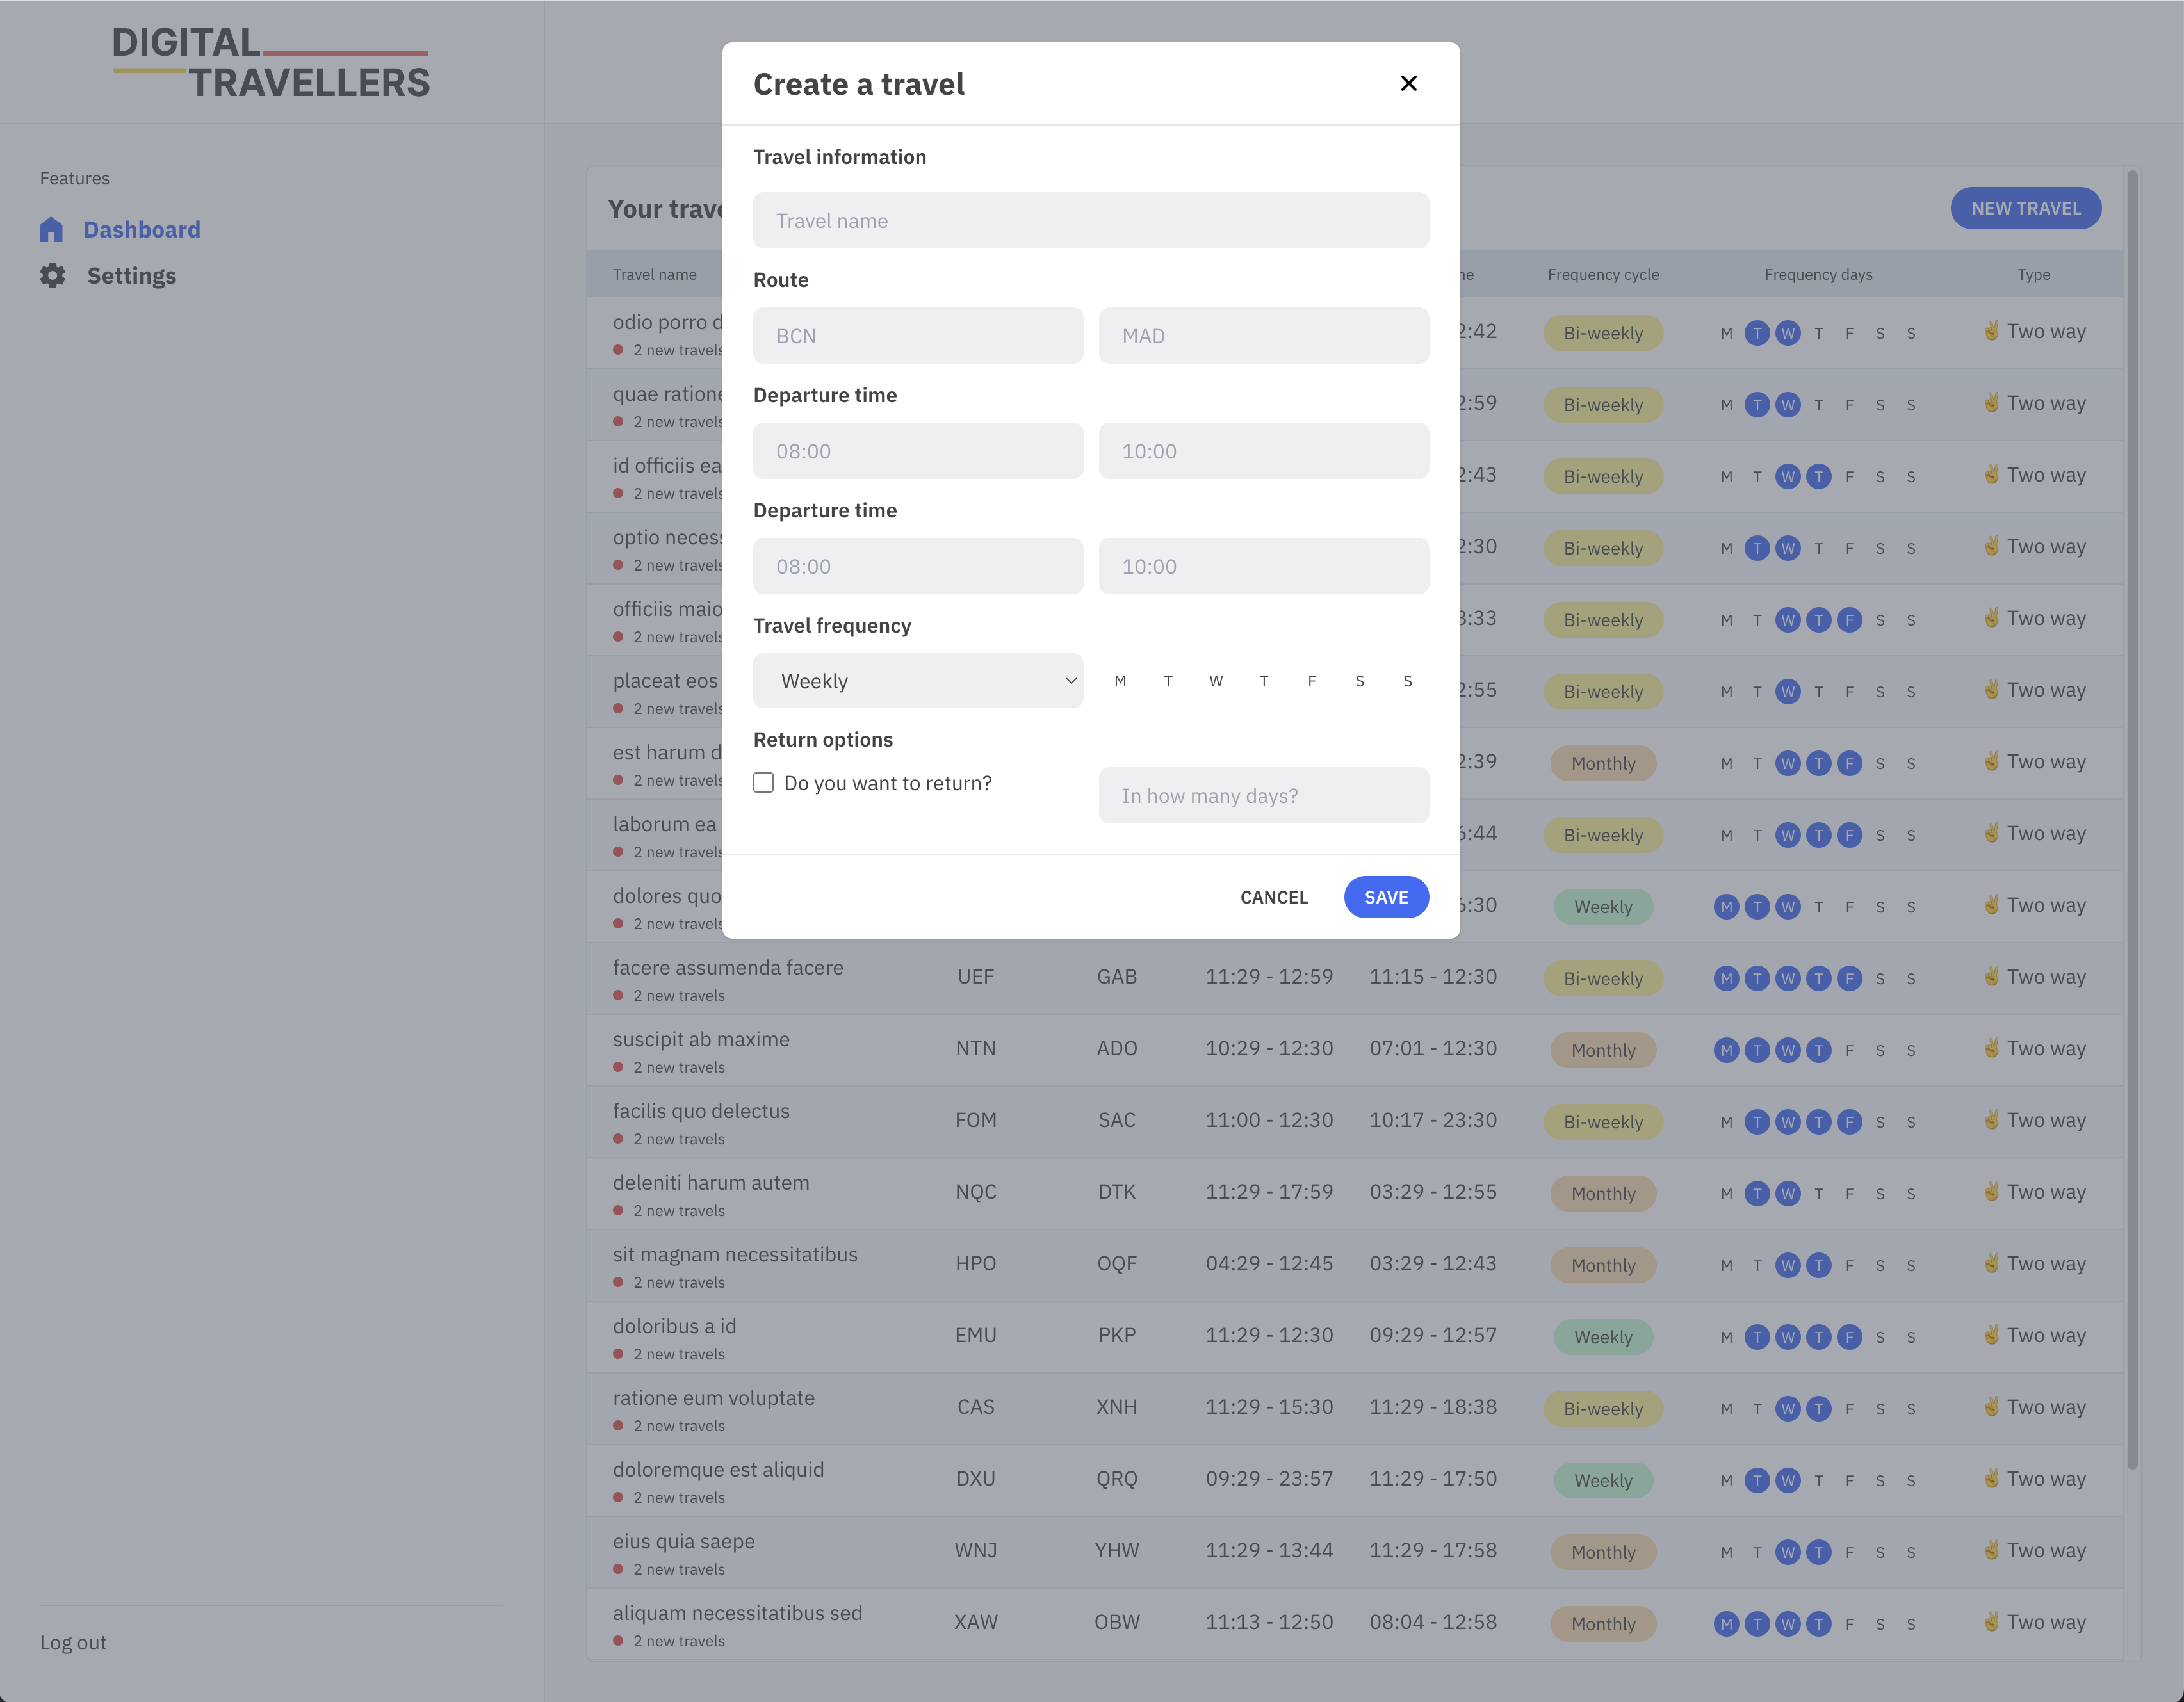
\includegraphics[width=\textwidth]{./assets/results/desktop-create.png}
	\caption{Final result of the dashboard page, when the dialog to create
		travels has been opened, for desktop devices}
\end{figure}
\begin{figure}[H]
	\centering
	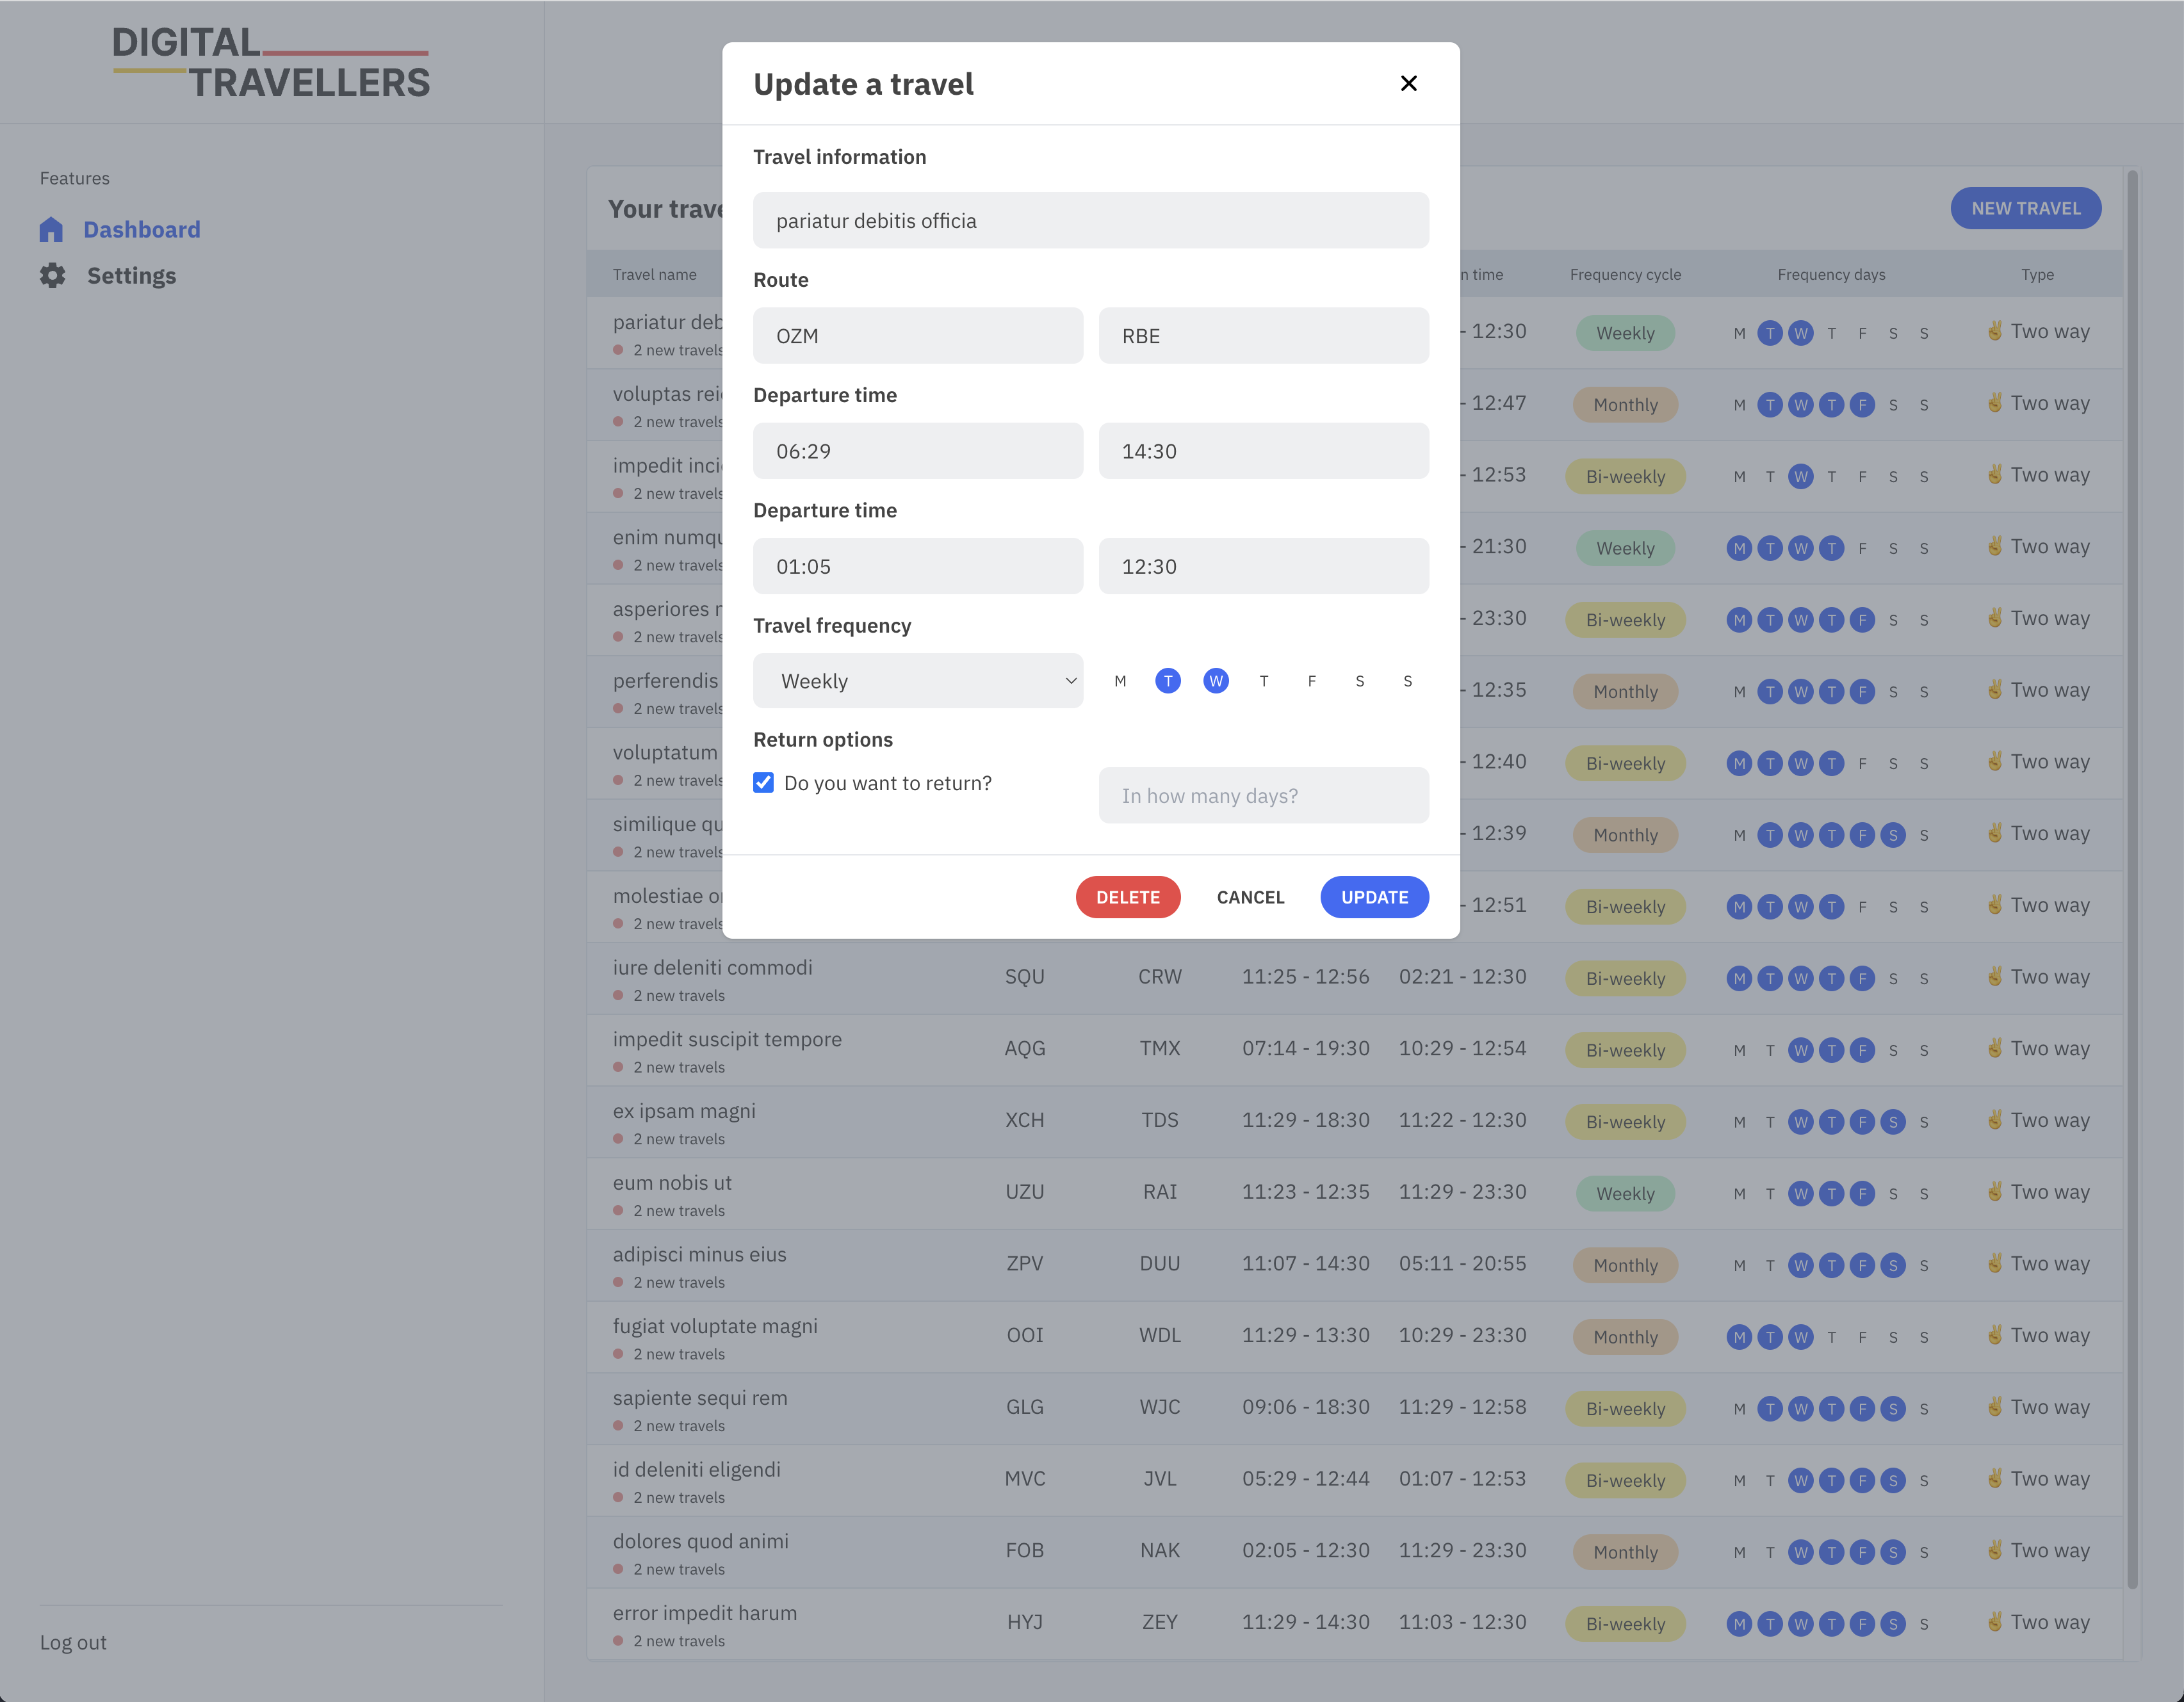
\includegraphics[width=\textwidth]{./assets/results/desktop-update.png}
	\caption{Final result of the dashboard page, when the dialog to create
		travels has been opened, for desktop devices}
\end{figure}
\begin{figure}[H]
	\centering
	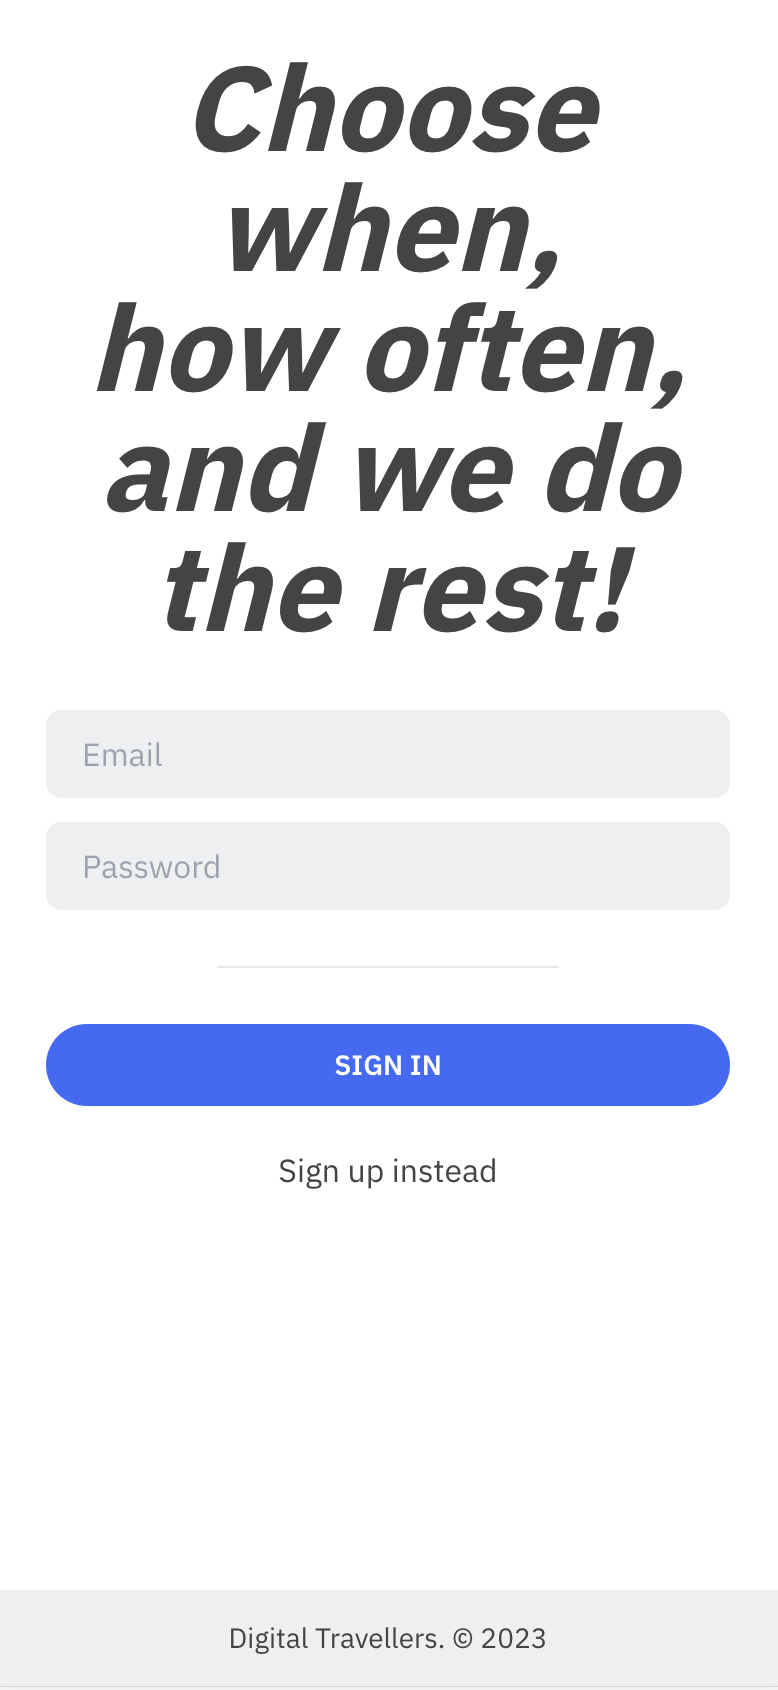
\includegraphics[width=0.25\textwidth]{./assets/results/mobile-sign-in.png}
	\hspace*{12pt}
	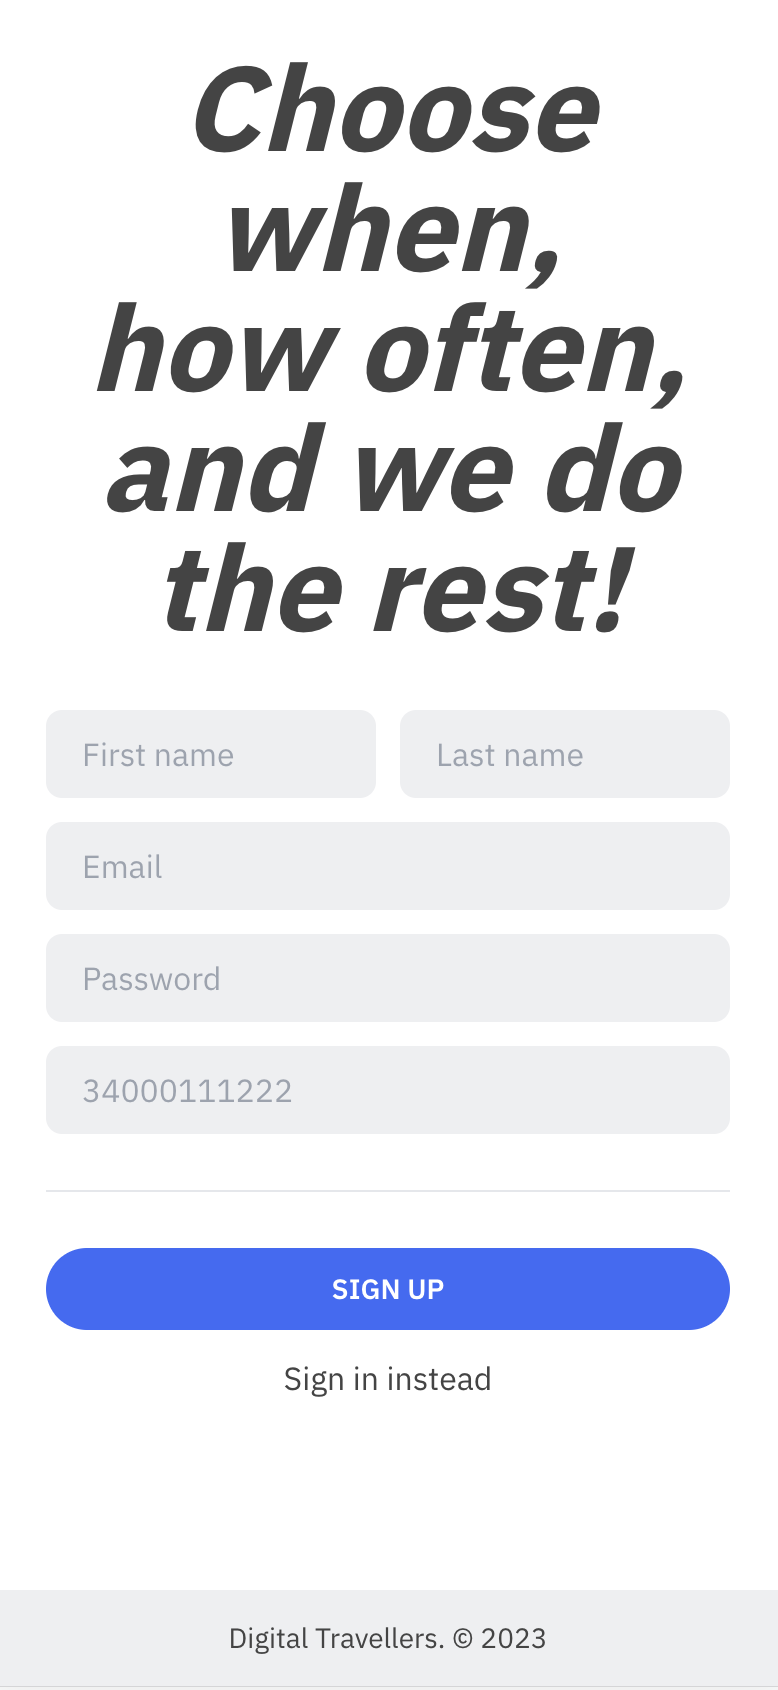
\includegraphics[width=0.25\textwidth]{./assets/results/mobile-sign-up.png}
	\hspace*{12pt}
	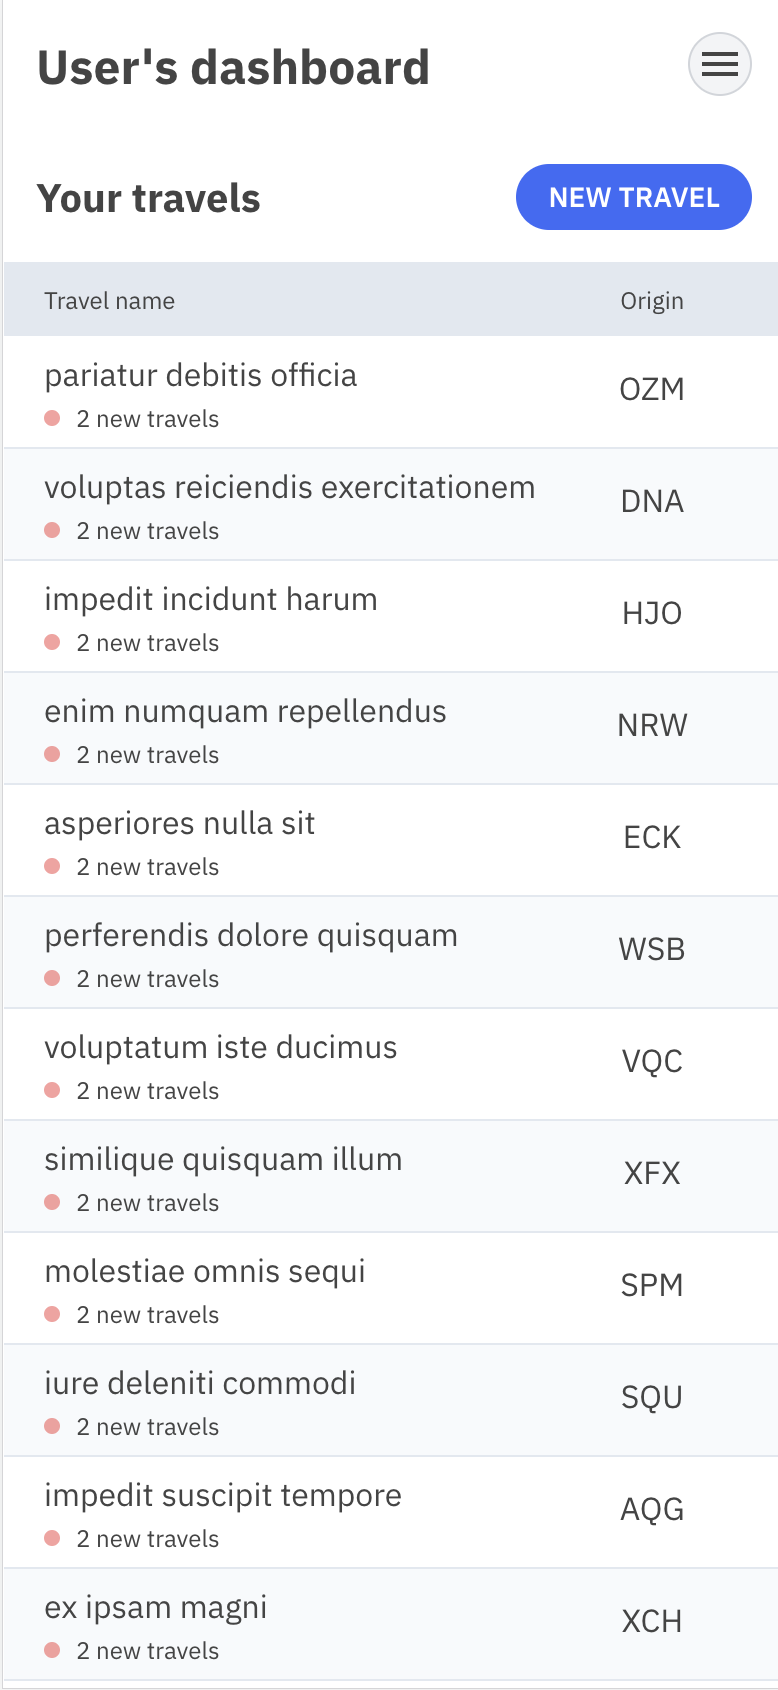
\includegraphics[width=0.25\textwidth]{./assets/results/mobile-dashboard.png}
	\caption{From left to right, all for mobile devices; Final result of the
		sign-in page. Final result of the sign-up page. Final result of the
		dashboard page (scrollable).}
\end{figure}
\begin{figure}[H]
	\centering
	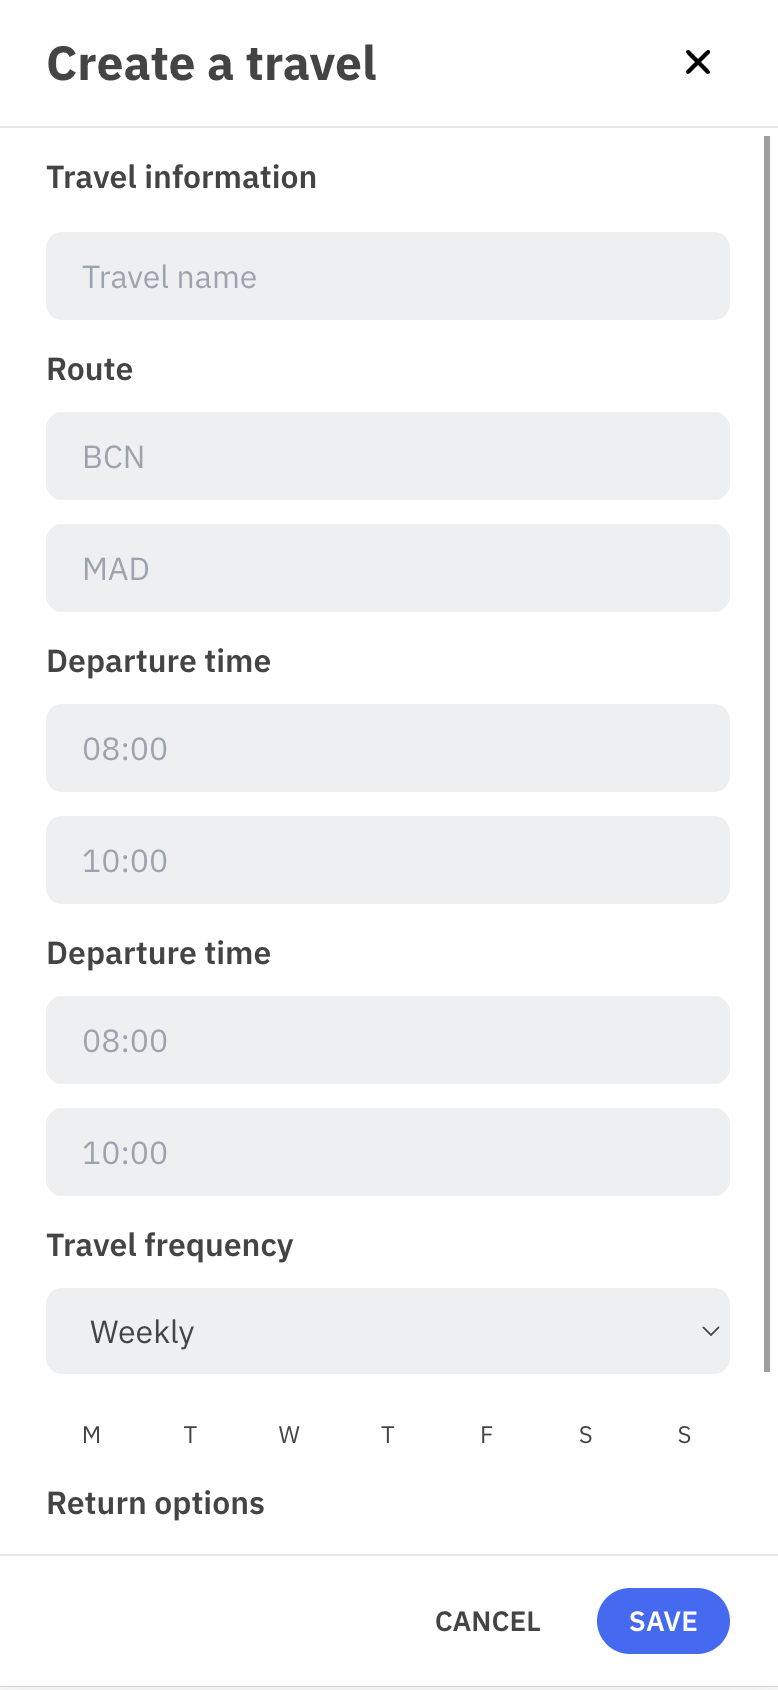
\includegraphics[width=0.25\textwidth]{./assets/results/mobile-create.png}
	\hspace*{12pt}
	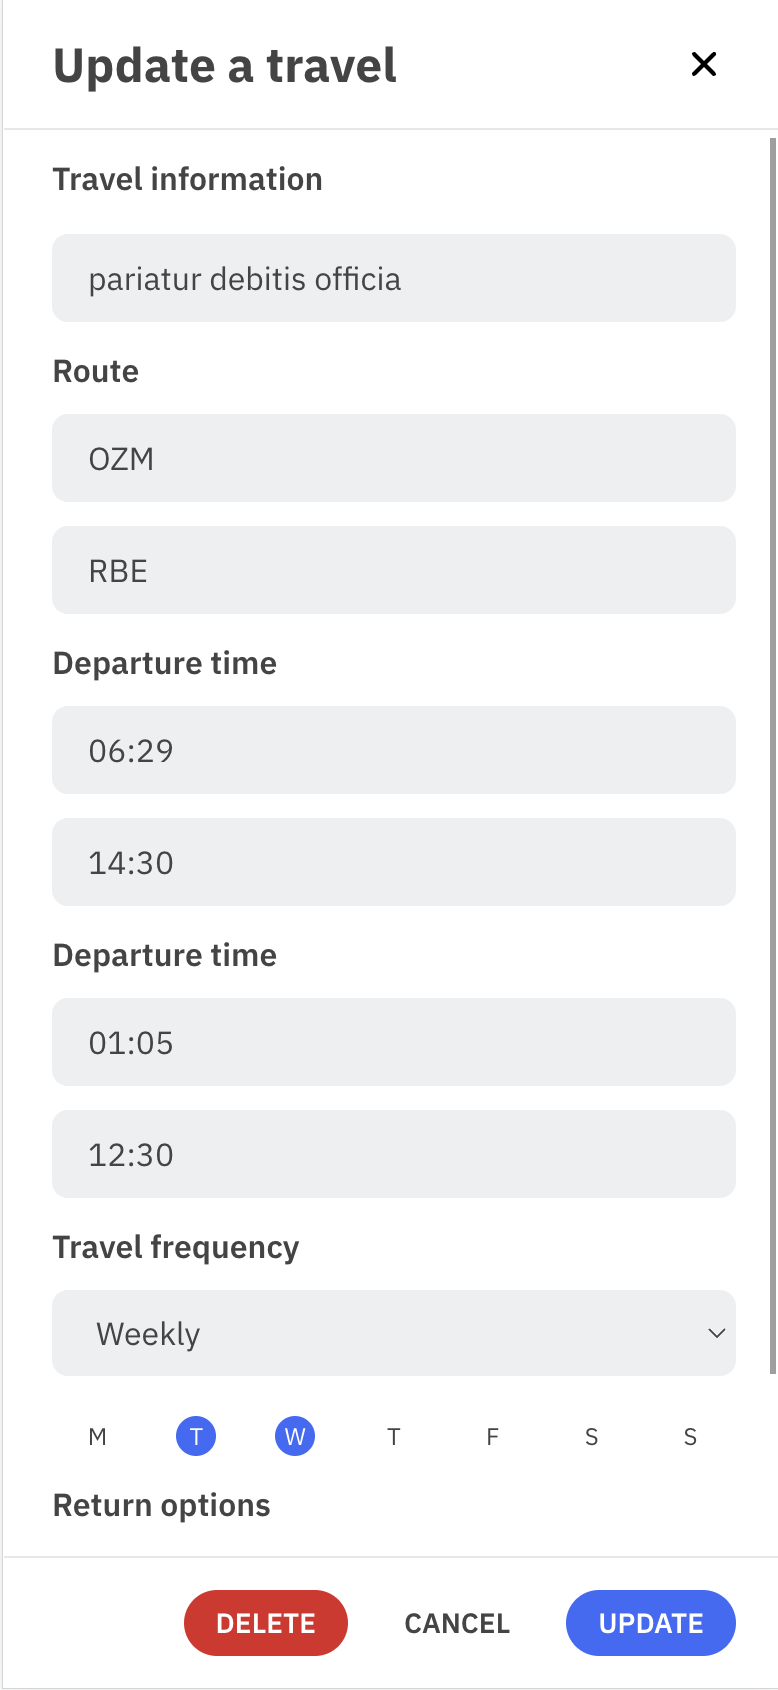
\includegraphics[width=0.25\textwidth]{./assets/results/mobile-update.png}
	\caption{From left to right, all for mobile devices; Final result of the
		dashboard when the dialog to create an alert has been opened. Final result
		of dashboard when the dialog to update an alert has been opened.}
\end{figure}
Both the live application and the attached pictures clearly demonstrate that the
final product provides a user interface that is not only simple and intuitive
but also clean and visually appealing. Moreover, the application exhibits
satisfactory performance, making it suitable for an MVP. The careful
craftsmanship of the designs has played a crucial role in ensuring consistency
and coherence in the user interface throughout the entire application.
\\[8pt]
In future work, the adoption of Domain-Driven Design (DDD), hexagonal
architecture, and SOLID principles will greatly benefit the project. DDD
emphasizes structuring the software around the core domain, enabling a clear
understanding of the business requirements and facilitating easier maintenance
and extensibility. By employing hexagonal architecture, the application can be
decoupled from external dependencies, making it more flexible and allowing for
easier integration of new features or technologies. Additionally, adhering to
SOLID principles promotes modularity, reusability, and testability of the
codebase, resulting in a more maintainable and robust system. These approaches
collectively contribute to better scalability, maintainability, and adaptability
of the application in the long run.
\end{document}
